\chapter{シミュレーションにおける実験評価}\label{simulation}

この章では,実験が適切に構築されているか,そしてその際に得られるべき物理量をMonte Carloシミュレーションを用いて評価する.


\section{シミュレーションの意義}

我々の実験では,複雑に物体が組み合わされており,我々が求めるイベントがどれくらいの頻度で発生しうるのかを計算するのは立体角や断面積の計算が入り組みかなり難しい.
そこでMonte Carloシミュレーションを用いて,実験レートを評価する.Geant4を用いてプラスチックシンチレータの中で停止せずに陽電子がターゲットに到達するか,そしてターゲットから発生したガンマ線がNaIシンチレータを光らせるかを確かめることができる.

今回用いた線源は$\ce{^{22}Na}$ の標準線源であり,200 kBqのものである.
この線源強度と我々の実験期間約1週間を考慮して,0.1 Hzの実験レートを目標に実験のデザインが適当か検証した.
本実験でオルソポジトロニウムの寿命を測定する過程の評価を,$\ce{^{22}Na}$ 線源が$\beta$ 崩壊した陽電子がシンチレーターを通過してシリカゲルに到達する過程のレート評価,線源から直接NaIシンチレータに入る$\gamma$ 線の評価,そして形成されたポジトロニウムが崩壊し,放出された$\gamma$ 線がNaIシンチレータで落とすエネルギーの評価の3つに分割してシミュレーションを行った.



\section{プラスチックシンチレーターの通過}

\subsection{概要}
今回の実験で用いられたプラスチックシンチレータは0.15 mmの厚みのものである.線源から放出される陽電子が,シンチレータ内で停止してしまうとシリカゲルに到達せずポジトロニウムを形成することができない.
ポジトロニウムを形成するためには,陽電子がまず標準線源のアルミ窓を通過して,空気中を伝播し,さらにシンチレータをエネルギーを落としきること無く通過する必要がある.
Geant4を用いて実際の線源を含めたジオメトリを作成し,シンチレータと線源の距離を変えながらエネルギーを落としきらず通過してくる粒子の割合を調べた.
このとき,ポジトロニウムのミキシングを起こすために用いる磁場を,陽電子をシリカゲルまで導く用途にも援用する.このときの磁場を,最もターゲットであるシリカゲルまで陽電子を導くのに効率が良い線源窓に垂直な方向に設定し,一様な磁場で強度は定格である0.1 Teslaと見積もった.この強度については後に考察する.

\subsection{ジオメトリ}

\begin{figure}[htbp]
	\centering
		\includegraphics[width=10cm]{img/test1_geo.png}
	\caption{構築したジオメトリ}
	\label{test1_geo}
\end{figure}

図\ref{test1_geo} はプラスチックシンチレーターの試験として作成したジオメトリで,標準線源とその表面から距離$d$離れたシンチレータ$\phi8$ mm,厚み0.15 mmのプラスチックシンチレーター,その直後に置かれた理想的な粒子検出器で構成されている.標準線源はデータシートにしたがって作成し,アクリルのケースと0.1 mm厚のアルミニウム製の窓を実装してある.理想的な粒子検出器は入射した粒子の種類とエネルギーが分解能無限大で確実にわかる.
\ce{^{22}Na}はbranching ratioにしたがって$\beta^+$崩壊する.

\subsection{陽電子到達数と立体角}

プラスチックシンチレーターを線源から遠くに置くほど,透過する陽電子数は減少すると考えられる.この減少には,空気中を伝播する際に陽電子が相互作用することも影響すると考えられるが,大部分の影響は立体角の減少に由来すると予想される.今回は理想的な粒子検出器を実装しているため,ニュートリノの数を調べることでも立体角を概算する事ができる.無論,立体角$\Omega$を解析的に計算することも今回は可能で,

\begin{equation}
	\Omega = 2\pi \left( 1-\cos\left(\arctan\frac{8/2}{d+2.5}\right)\right)
\end{equation}

で与えられる.今回は$d$を線源の表面からシンチレーターを通過するまでの距離と定義しているので,放射線源中心からの補正2.5 mmを加えている.

\subsection{磁場の援用}
概要でも触れたが,ポジトロニウムのミキシングを起こさせるための磁場を,陽電子をターゲットまで導くことにも援用することができる.
図\ref{mag_effect}で磁場のあるジオメトリで線源からの粒子を視覚化した.青の軌跡が陽電子,赤の軌跡が電子で\ce{^{22}Na}を1,000個崩壊させている
強力に磁場方向に引き寄せられるのが見て取れるので,磁場をかけたとき,かけないときでレートを比較する.

\begin{figure}[htbp]
	\centering
		\includegraphics[width=10cm]{img/mag_effect.png}
	\caption{磁場をかけた状態での粒子軌跡の視覚化}
	\label{mag_effect}
\end{figure}


\subsection{結果}

図\ref{scinti_test}がシンチレーターを陽電子が通過する割合の距離依存である.

\begin{figure}[htbp]
	\centering
		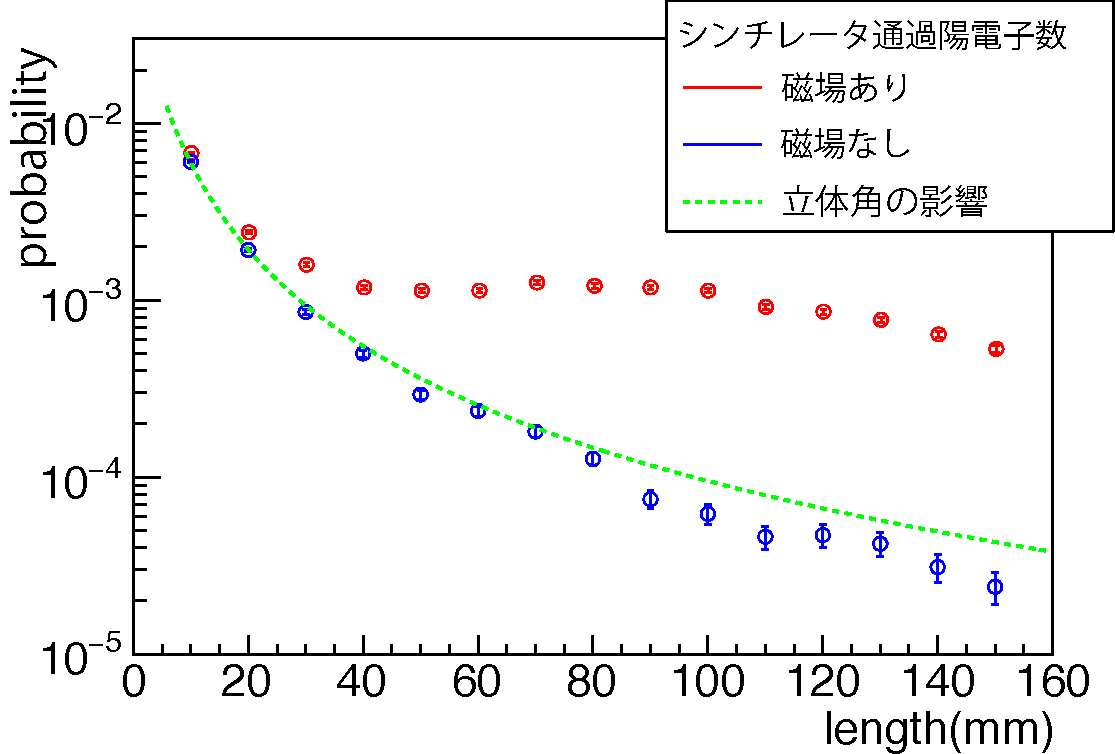
\includegraphics[width=10cm]{fig/scinti_test.pdf}
	\caption{プラスチックシンチレータ通過粒子割合}
	\label{scinti_test}
\end{figure}

\subsection{考察}

ほとんど物質と相互作用せず,等方的に放出されることが予想されるニュートリノの到達数と,解析的に求められた立体角がエラーの範囲でよく一致することは明らかである.
これは,Geant4のジオメトリが正しく作製されていることを示している.
一方で,磁場をかけたときとかけていないときで,陽電子の到達数には差がある,


\section{崩壊陽電子に対するバックグラウンド評価}

\subsection{ジオメトリ}

\section{予想されるエネルギースペクトル}

